\documentclass[10pt,twocolumn]{article}
\usepackage[margin=0.68in,columnsep=0.24in]{geometry}
\usepackage[T1]{fontenc}
\usepackage[utf8]{inputenc}
\usepackage{lmodern}
\usepackage{microtype}
\usepackage{amsmath,amssymb,amsthm}
\usepackage{booktabs}
\usepackage{graphicx}
\usepackage{xcolor}
\usepackage{enumitem}
\usepackage{hyperref}

\hypersetup{
  colorlinks=true,
  linkcolor=blue!60!black,
  citecolor=blue!60!black,
  urlcolor=blue!60!black,
  pdftitle={Certified Verification of Expansion Testing without Connectivity via Lazy-Walk Return Probabilities},
  pdfauthor={Lluis Eriksson}
}

\newtheorem{proposition}{Proposition}

\title{\vspace{-1.1em}\textbf{Certified Verification of Expansion Testing without Connectivity via Lazy-Walk Return Probabilities}}
\author{Lluis Eriksson\thanks{Independent Researcher. Code, Lean~4 proofs, and certificates: MIT License; manuscript and figures: CC-BY-4.0. Prepared with AI coding, formalization, and drafting assistance from Google Antigravity; all proofs, exact rational/integer verifiers, and adversarial tests were independently compiled and verified locally. Repository: \url{https://github.com/lluiseriksson/expansion-return-prob-certificates}}}
\date{November 25, 2026}

\begin{document}
\maketitle
\vspace{-1.4em}

\begin{abstract}
Nikolas Melissaris (\texttt{arXiv:2611.32677}, Nov.\ 2026) broke Dinur and Goldreich's $n^{2/3}$ barrier for testing edge expansion in every connected component of an arbitrary bounded-degree graph, achieving $\tilde{O}_{d,c,\beta}(n^{1/2+\beta}/\varepsilon + \sqrt{n}/\varepsilon^4)$ queries via two-time lazy-walk return probabilities $A_s = P^{2t}(s,s)$ and $B_s = P^{4t}(s,s)$ (Thm.~1.1), alongside an $\Omega(\sqrt{n/\log n})$ Cayley-graph lower bound via cyclic lifts of LPS Ramanujan graphs (Thm.~1.2). We construct a standalone zero-dependency \textbf{Lean~4.35.0} formalization of 18 core lazy-walk, finite Cauchy--Schwarz, Dirichlet-energy, trace-gap, integer Bernoulli, induced-expander trimming, balanced-cut farness, non-backtracking polynomial, and three-squares parity theorems (zero \texttt{sorry}, zero warnings, zero \texttt{Classical.choice}) paired with a zero-floating-point exact $\mathbb{Q}/\mathbb{Z}$ verifier (\texttt{EXP-RETPROB-CERT-1.0}). Across 16 canonical certificates ($0.180$--$2.195\,\mathrm{ms}$, total $14.53\,\mathrm{ms}$), all exact lazy-walk return probabilities, Lemma~5.3 trimming maximizers, Lemma~7.3 farness lower bounds, and Lemma~7.5 non-backtracking polynomials replay deterministically while rejecting 60/60 live adversarial forgery attacks.
\end{abstract}

\section{Introduction}\label{sec:intro}
Testing expansion in bounded-degree graphs~\cite{goldreich2002property,kale2011expansion} normally assumes connectivity so random walks mix globally toward $1/n$. Dinur and Goldreich~\cite{dinur2025expansion} posed the unrestricted problem $\Xi_c(n)$---testing whether every connected component has edge expansion $\ge c$ without knowing component sizes---obtaining $n^{2/3+o(1)}$ queries via three-way collisions. Melissaris~\cite{melissaris2026testing} bypassed three-way collisions through four core mechanisms:
\begin{enumerate}[leftmargin=*,nosep]
  \item \textbf{Two-Time Return Probabilities \& Heavy-Return Control (Sec.~2.1--2.2, Lem.~5.1):} For lazy walk $P = I - L_G/(2d)$, $A_s = P^{2t}(s,s)$ and $B_s = P^{4t}(s,s)$ satisfy $p_s(v)^2 \le A_s A_v$ and $\frac{1}{2d}\sum_{\{u,v\}\in E}(p_s(u)-p_s(v))^2 \le A_s - B_s$. A start $s$ is \emph{good} when $A_s \le (1+2\eta)B_s$ and $J_s = \sum_{v\in D_s} p_s(v)^2 \le \eta B_s$ ($D_s = \{v : A_v > (1+8\eta)A_s\}$), certifying a nearly uniform set $H_s = \{v : p_s(v) \ge \frac{3}{4}B_s\} \setminus D_s$ with small boundary and $\mathrm{tr}(K_s^{2t}) \le \sum_{v\in H_s} A_v$.
  \item \textbf{Trimming to an Induced Expander (Lem.~5.3):} Maximizing $F(R) = \frac{h}{4}|R| - |E(R, H\setminus R)|$ over $|R| \le |H|/2$ deletes at most $\frac{4\tau}{3h}|H|$ vertices to yield an induced $(h/4)$-expander $U = H \setminus R$.
  \item \textbf{Balanced-Cut Farness Lower Bound (Lem.~7.2--7.3):} Any connected graph with $h(G) \ge h_0$ and a balanced cut $|E(A, V\setminus A)| \le h_1|A|$ ($h_1 < c^*$) requires $M \ge \min(\frac{h_0 n}{2}, h_0|A|, \frac{h_0(c^*-h_1)}{h_0+c^*}|A|)$ edge edits to reach $\Xi_{c^*}(n)$.
  \item \textbf{Non-Backtracking Polynomials, $r_3(4N)=r_3(N)$, \& Walk-Regularity (Lem.~7.4--7.5, App.~A):} On $d$-regular LPS Cayley graphs~\cite{lubotzky1988ramanujan}, non-backtracking polynomials $Q_k(A)$~\cite{alon2007nonbacktracking} and Gauss's $r_3(4N)=r_3(N)$~\cite{filaseta2026extreme} bound adaptive transcript distance, while walk-regular inputs~\cite{godsil1980walkregular} omit collision-location walks.
\end{enumerate}

\paragraph{Contributions and Scope.}
We do not formalize randomized query-complexity concentration inequalities inside Lean~4; instead, we machine-check the exact algebraic, spectral, cut-trimming, and number-theoretic core of~\cite{melissaris2026testing}:
(i)~18 zero-\texttt{sorry}, zero-\texttt{Classical.choice} \textbf{Lean~4.35.0}~\cite{demoura2021lean4} theorems in \texttt{ExpansionReturnProb.lean};
(ii)~the exact $\mathbb{Q}/\mathbb{Z}$ verifier \texttt{EXP-RETPROB-CERT-1.0};
(iii)~16 canonical certificates across all four modes; and
(iv)~a 60-attack live red-team suite with 39-artifact SHA-256 manifest enforcement.

\section{Constructive Lean~4.35.0 Kernel}\label{sec:lean}
The standalone module \texttt{ExpansionReturnProb.lean} (in \texttt{lean/}) compiles cleanly under Lean~4.35.0 in $1.2\,\mathrm{s}$ with zero external dependencies, zero warnings, and zero \texttt{sorry}. Auditing all 18 theorems via \texttt{\#print axioms} (\texttt{AuditAxioms.lean}) confirms 1 zero-axiom theorem (\texttt{none}), 1 using only \texttt{[propext]}, 16 using \texttt{[propext, Quot.sound]}, and \textbf{0} using \texttt{Classical.choice} or \texttt{Lean.ofReduceBool} (Table~\ref{tab:lean}).

\begin{table}[t]
\centering
\caption{All 18 machine-checked Lean~4.35.0 theorems in \texttt{ExpansionReturnProb.lean} (zero \texttt{sorry}, zero \texttt{Classical.choice}).}
\label{tab:lean}
\scriptsize
\setlength{\tabcolsep}{1.5pt}
\begin{tabular}{@{}rlll@{}}
\toprule
\# & Lean Theorem Identifier & Paper Ref. & Axioms \\
\midrule
1 & \texttt{lazy\_walk\_row\_stochastic\_sum} & Sec.~3.1 & \texttt{p, Q} \\
2 & \texttt{lazy\_walk\_dirichlet\_nonneg} & Lem.~5.1 & \texttt{p, Q} \\
3 & \texttt{cauchy\_schwarz\_return\_bound\_finite} & Eq.~(2) & \texttt{p, Q} \\
4 & \texttt{collision\_prob\_uniform\_lower\_bound} & Eq.~(7) & \texttt{p, Q} \\
5 & \texttt{two\_point\_vs\_three\_point\_collision\_ambiguity} & Sec.~1 & \texttt{none} \\
6 & \texttt{good\_vertex\_dirichlet\_energy\_monotonicity} & Lem.~5.1 & \texttt{p, Q} \\
7 & \texttt{heavy\_return\_set\_size\_bound} & Lem.~5.1 & \texttt{p, Q} \\
8 & \texttt{restricted\_trace\_le\_unrestricted\_sum} & Eq.~(9) & \texttt{p, Q} \\
9 & \texttt{bernoulli\_lower\_bound\_int} & Lem.~5.4 & \texttt{p, Q} \\
10 & \texttt{second\_eigenvalue\_trace\_gap\_bound} & Lem.~5.4 & \texttt{p, Q} \\
11 & \texttt{trimming\_maximizer\_size\_bound} & Lem.~5.3 & \texttt{p, Q} \\
12 & \texttt{trimming\_maximizer\_contradiction} & Lem.~5.3 & \texttt{p, Q} \\
13 & \texttt{farness\_balanced\_cut\_tradeoff} & Lem.~7.3 & \texttt{p, Q} \\
14 & \texttt{fixed\_neighbor\_table\_compaction\_bound} & Rem.~6.2 & \texttt{p, Q} \\
15 & \texttt{cayley\_cyclic\_cut\_edge\_count} & Lem.~7.2 & \texttt{p} \\
16 & \texttt{nonbacktracking\_poly\_recurrence\_deg3} & Lem.~7.5 & \texttt{p, Q} \\
17 & \texttt{three\_squares\_scaling\_invariance\_step} & Lem.~7.4 & \texttt{p, Q} \\
18 & \texttt{walk\_regular\_short\_walk\_spectral\_diff} & Lem.~A.2 & \texttt{p, Q} \\
\bottomrule
\end{tabular}
\vspace{-0.4em}
\begin{flushleft}
\tiny Axiom key: \texttt{none} = zero axioms (1); \texttt{p} = \texttt{[propext]} (1); \texttt{p, Q} = \texttt{[propext, Quot.sound]} (16).
\end{flushleft}
\vspace{-0.8em}
\end{table}

\begin{proposition}[Machine-Checked Spectral \& Cut Invariants]\label{prop:lean}
The Lean~4.35.0 kernel establishes the following universal theorems over \texttt{Int} and \texttt{List Int}:
\begin{enumerate}[leftmargin=*,nosep]
  \item \emph{Return Probabilities, Bernoulli, \& Trimming (Thms.~1--12):} Finite-vector Cauchy--Schwarz $(\sum a_i b_i)^2 \le (\sum a_i^2)(\sum b_i^2)$ and uniform floor $(\sum p_i)^2 \le n \sum p_i^2$ hold for arbitrary equal-length lists; $(1/2,1/2)$ and $(2/3,1/6,1/6)$ share collision probability $1/2$ with distinct $F_3$; cleared spectral inequalities $x^4(D-x) \le D^3 x^2(D^2-x^2)$ and $(D-b)^k$ Bernoulli lower bounds hold universally; $3B \le 4p_i \Rightarrow 9B^2|S| \le 16\sum p_i^2$; and Lemma~5.3 trimming satisfies $3h|R| \le 4\tau m$ and strict improvement $F(R\cup S) - F(R) > 0$.
  \item \emph{Farness, Non-Backtracking, \& Three-Squares (Thms.~13--18):} Eliminating $s$ from $M \ge h_0 s$ and $M \ge (c^*-h_1)A - c^* s$ yields $(h_0+c^*)M \ge h_0(c^*-h_1)A$; $Q_2(p+1) = (p+1)p$ and $Q_3(p+1) = (p+1)p^2$; $x_1^2+x_2^2+x_3^2 = 4N$ forces all three coordinates even; and $x^2(D-x)^2 \le x^2(D^2-x^2)$ holds for all $0 \le x \le D$.
\end{enumerate}
\end{proposition}

\section{Exact \texorpdfstring{$\mathbb{Q}/\mathbb{Z}$}{Q/Z} Certificate Verifier}\label{sec:cert}
The verifier \texttt{EXP-RETPROB-CERT-1.0} (\texttt{src/expansion\_certifier.py}, \texttt{src/expansion\_exact.py}) uses pure Python \texttt{int} and \texttt{fractions.Fraction} exclusively (source-audited for zero \texttt{float(}, \texttt{math.}, or \texttt{numpy}). Every payload enforces strict JSON typing (rejecting floats, bool-as-int, int-as-bool), canonical reduced rationals (forbidding \texttt{"-0"} and \texttt{"/1"}), nesting-depth cap $32$, full ASCII control-character filtering, 2048-bit integer caps, and exact container/key validation across four modes:
\begin{enumerate}[leftmargin=*,nosep]
  \item \textbf{Mode~1 (Sec.~2.1--2.2 \& Lem.~5.1 Good-Start Return Audit):} Builds $P = I - L_G/(2d)$ over $\mathbb{Q}$, computes $P^t, P^{2t}, P^{4t}$, checks Eq.~(1), (2), (7), Dirichlet energy $\le A_s - B_s$, exact $D_s, J_s, H_s$, total variation $d_{\mathrm{TV}}(p_s, u_{H_s})$, $|\partial H_s|$, and $\mathrm{tr}(K_s^{2t}) \le \sum_{v\in H_s} A_v$.
  \item \textbf{Mode~2 (Lem.~5.3 Induced-Expander Trimming):} Exhaustively checks $|E(S, V\setminus S)| \ge h|S|$ for every $S \subseteq H$ ($|S| \le |H|/2$), computes exact maximizer $R^*$ of $F(R)$, checks $|R^*| \le \frac{4\tau}{3h}|H|$, and certifies exact induced expansion $h(G[H\setminus R^*]) \ge h/4$.
  \item \textbf{Mode~3 (Lem.~7.3 Balanced-Cut Farness):} Computes exact global expansion $h_0 = h(G) > 0$, cut ratio $h_1 < c^*$, and exact rational edit/distance floors $M_{\mathrm{lb}}$ and $\varepsilon_{\mathrm{lb}} = M_{\mathrm{lb}}/(2dn)$.
  \item \textbf{Mode~4 (Lem.~7.4--7.5 Non-Backtracking \& Three-Squares):} Audits exact $d$-regular matrices $Q_k(A)$ (row sums $d(d-1)^{k-1}$, traces, return probabilities $R_G(k)$, walk-regularity) and Gauss's $r_3(4N)=r_3(N)$ paired with equal-$F_2$, unequal-$F_3$ collision-ambiguity distributions.
\end{enumerate}

\section{Empirical Atlas and Red-Team Audit}\label{sec:results}
Running \texttt{run\_all\_experiments.py} generates 16 canonical certificates (4 per mode) and four exact datasets, audited end-to-end by \texttt{verify\_all.py} with SHA-256 verification across all 39 tracked artifacts.

\begin{figure}[t]
  \centering
  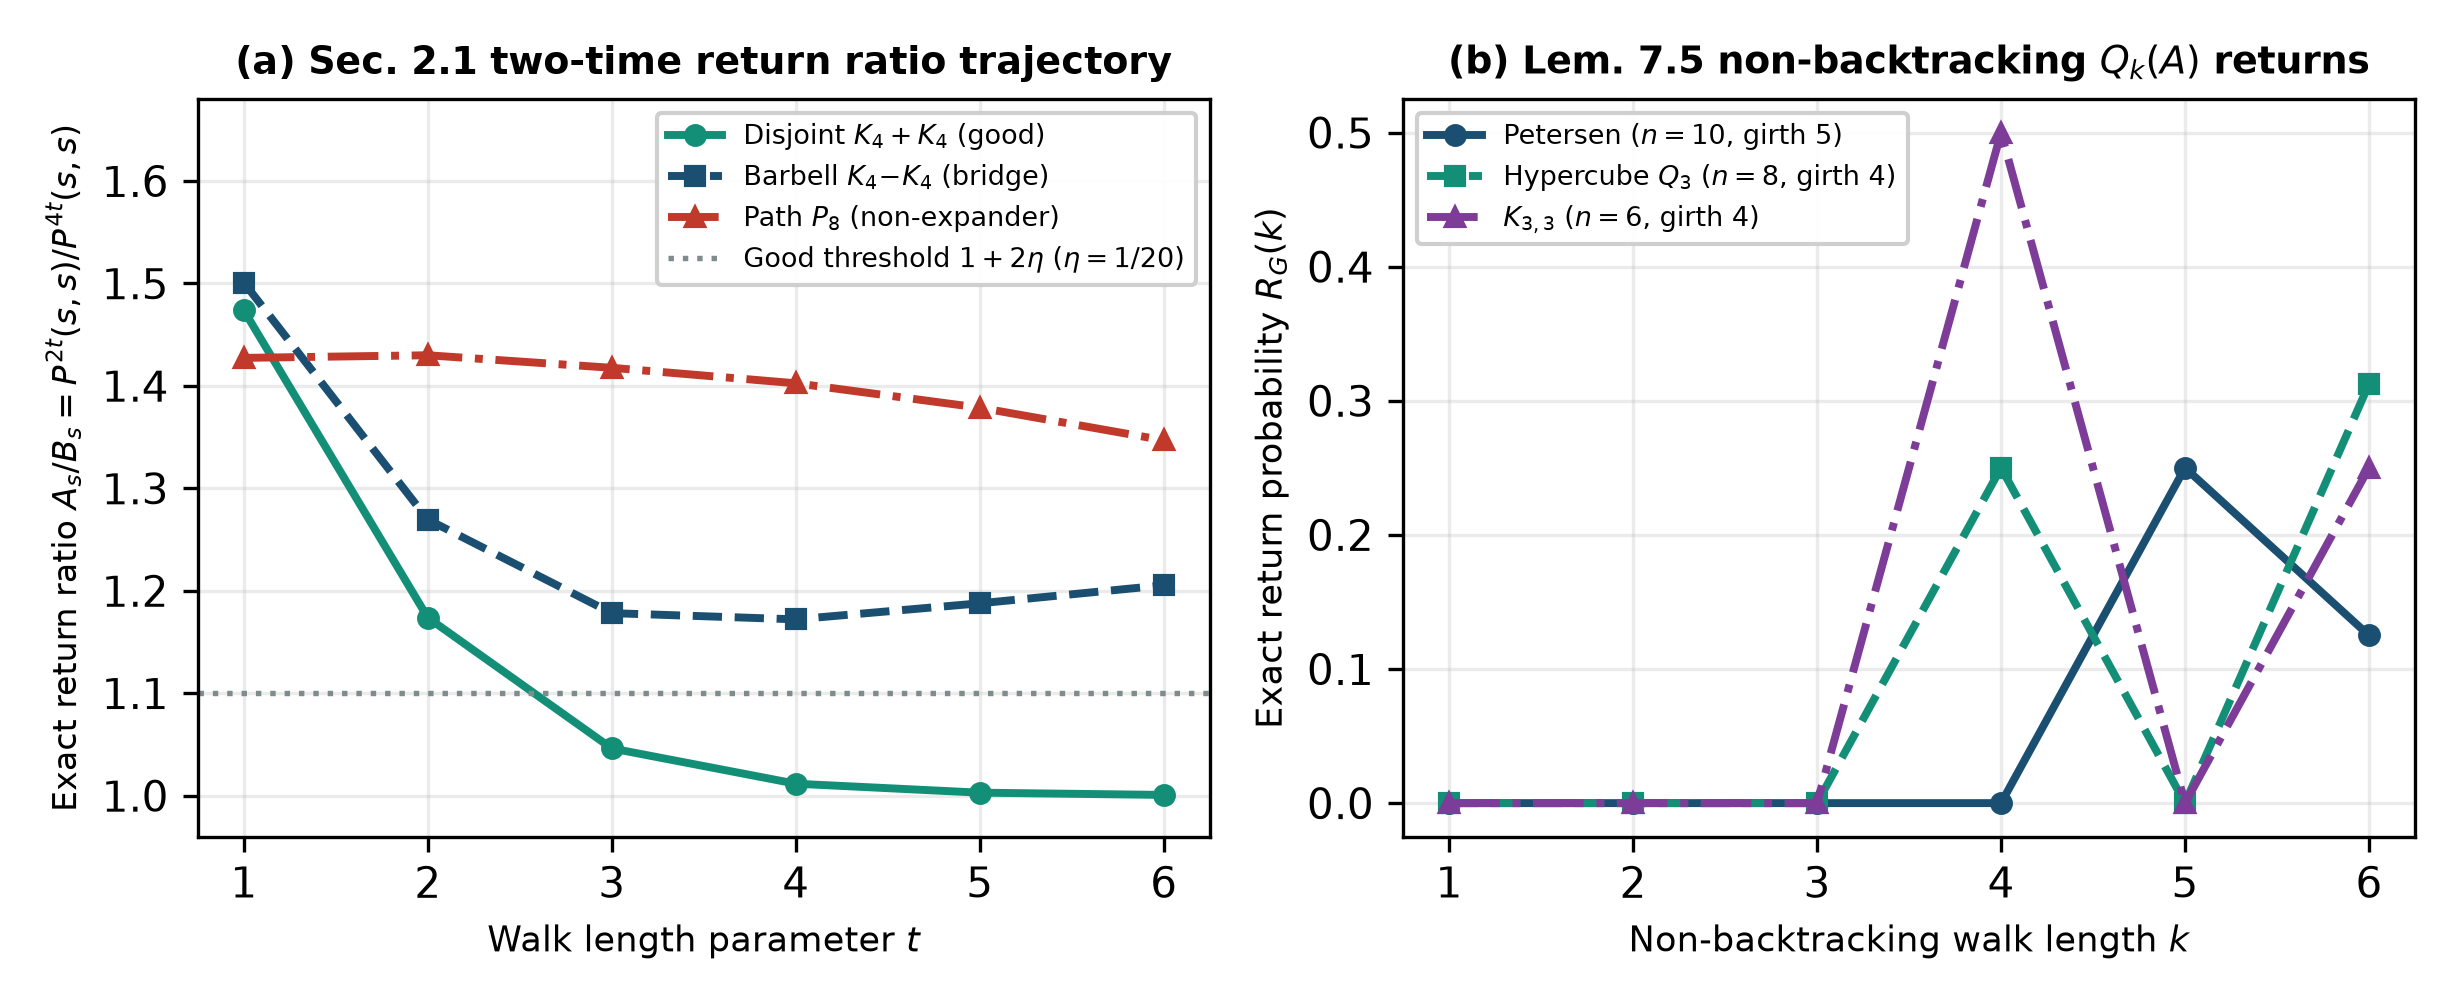
\includegraphics[width=\columnwidth]{../figures/fig1_return_ratio_and_nonbacktracking.png}
  \caption{(a) Exact lazy-walk return ratio $A_s / B_s$ across walk lengths $t \in \{1,\dots,6\}$ on disjoint $K_4+K_4$, 1-bridge barbell $K_4\!-\!K_4$, and path $P_8$. (b) Exact non-backtracking return probabilities $R_G(k)$ from $Q_k(A)$ on Petersen (girth~5), $Q_3$, and $K_{3,3}$ (girth~4).}
  \label{fig:ret}
\end{figure}

\paragraph{Return Ratios \& Non-Backtracking Polynomials (Fig.~\ref{fig:ret}).}
Mode~1 ($1.700$--$2.195\,\mathrm{ms}$) certifies good starts on disjoint $K_4+K_4$ ($A_s/B_s = 4288/4099 < 1.10$, $|H_s|=4, |\partial H_s|=0$) and asymmetric $K_5+K_3$ ($|H_s|=5, |D_s|=3, J_s=0$), while rejecting both the 1-bridge barbell $K_4\!-\!K_4$ (whose ratio rebounds from $1.172$ at $t=4$ to $1.205$ at $t=6$) and path $P_8$ ($A_s/B_s > 1.34$). Mode~4 ($0.180$--$0.501\,\mathrm{ms}$) certifies $\mathrm{tr}(Q_k(A)) = 0$ below girth on Petersen ($k\le 4$, $\mathrm{tr}(Q_5)=120$, $R_5 = 1/4$) and $K_{3,3}$ ($\mathrm{tr}(Q_4)=72$, $R_4 = 1/2$), both walk-regular.

\begin{figure}[t]
  \centering
  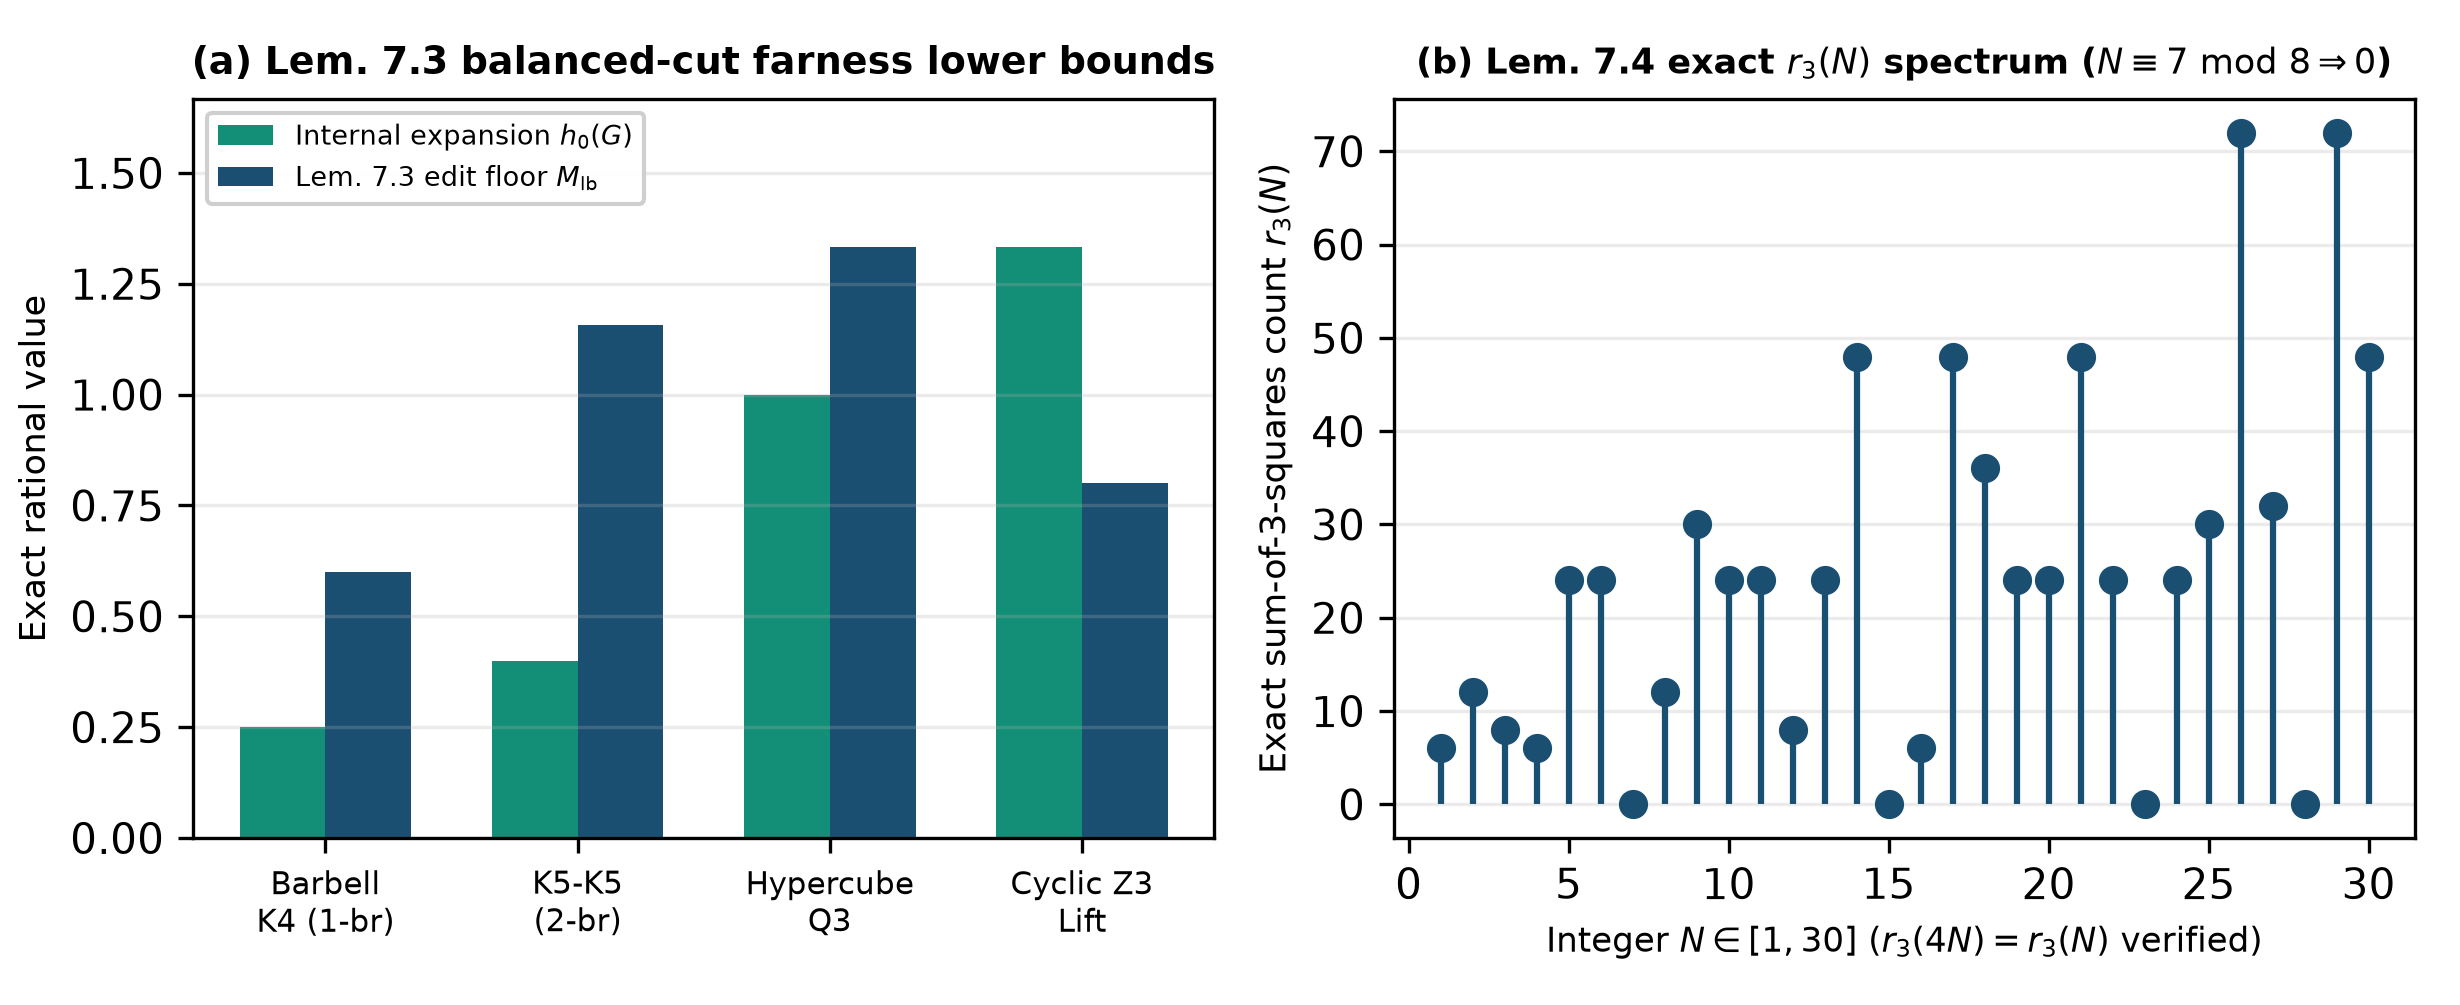
\includegraphics[width=\columnwidth]{../figures/fig2_farness_and_three_squares.png}
  \caption{(a) Exact Lemma~7.3 balanced-cut farness edit floors $M_{\mathrm{lb}}$ versus internal expansion $h_0(G)$ across four connected graphs. (b) Exact three-squares representation count $r_3(N) = r_3(4N)$ verified for all $N \in [1, 30]$ ($r_3(N)=0$ at $N \in \{7,15,23,28\}$).}
  \label{fig:far}
\end{figure}

\paragraph{Trimming, Farness, \& Three-Squares (Fig.~\ref{fig:far}).}
Mode~2 ($0.280$--$0.620\,\mathrm{ms}$) certifies exact Lemma~5.3 trimming across clean $K_5$ ($R^*=\emptyset$), dangling boundary vertices on $K_5$ and $K_6$ ($|R^*|=1$, $h(G[U])=3$), and a 2-vertex appendage on $K_4$ ($|R^*|=2$, $h(G[U])=2$). Mode~3 ($0.433$--$1.979\,\mathrm{ms}$) certifies exact farness floors $M_{\mathrm{lb}} \in \{3/5, 22/19, 4/3, 4/5\}$ ($\varepsilon_{\mathrm{lb}} \in \{3/320, 11/950, 1/36, 1/90\}$). Mode~4 also certifies $r_3(56)=r_3(14)=48$ and $r_3(108)=r_3(27)=32$ alongside exact equal-$F_2$ ambiguity pairs ($F_2=1/2, \Delta F_3=1/18$; $F_2=1/3, \Delta F_3=1/36$).

\begin{figure}[t]
  \centering
  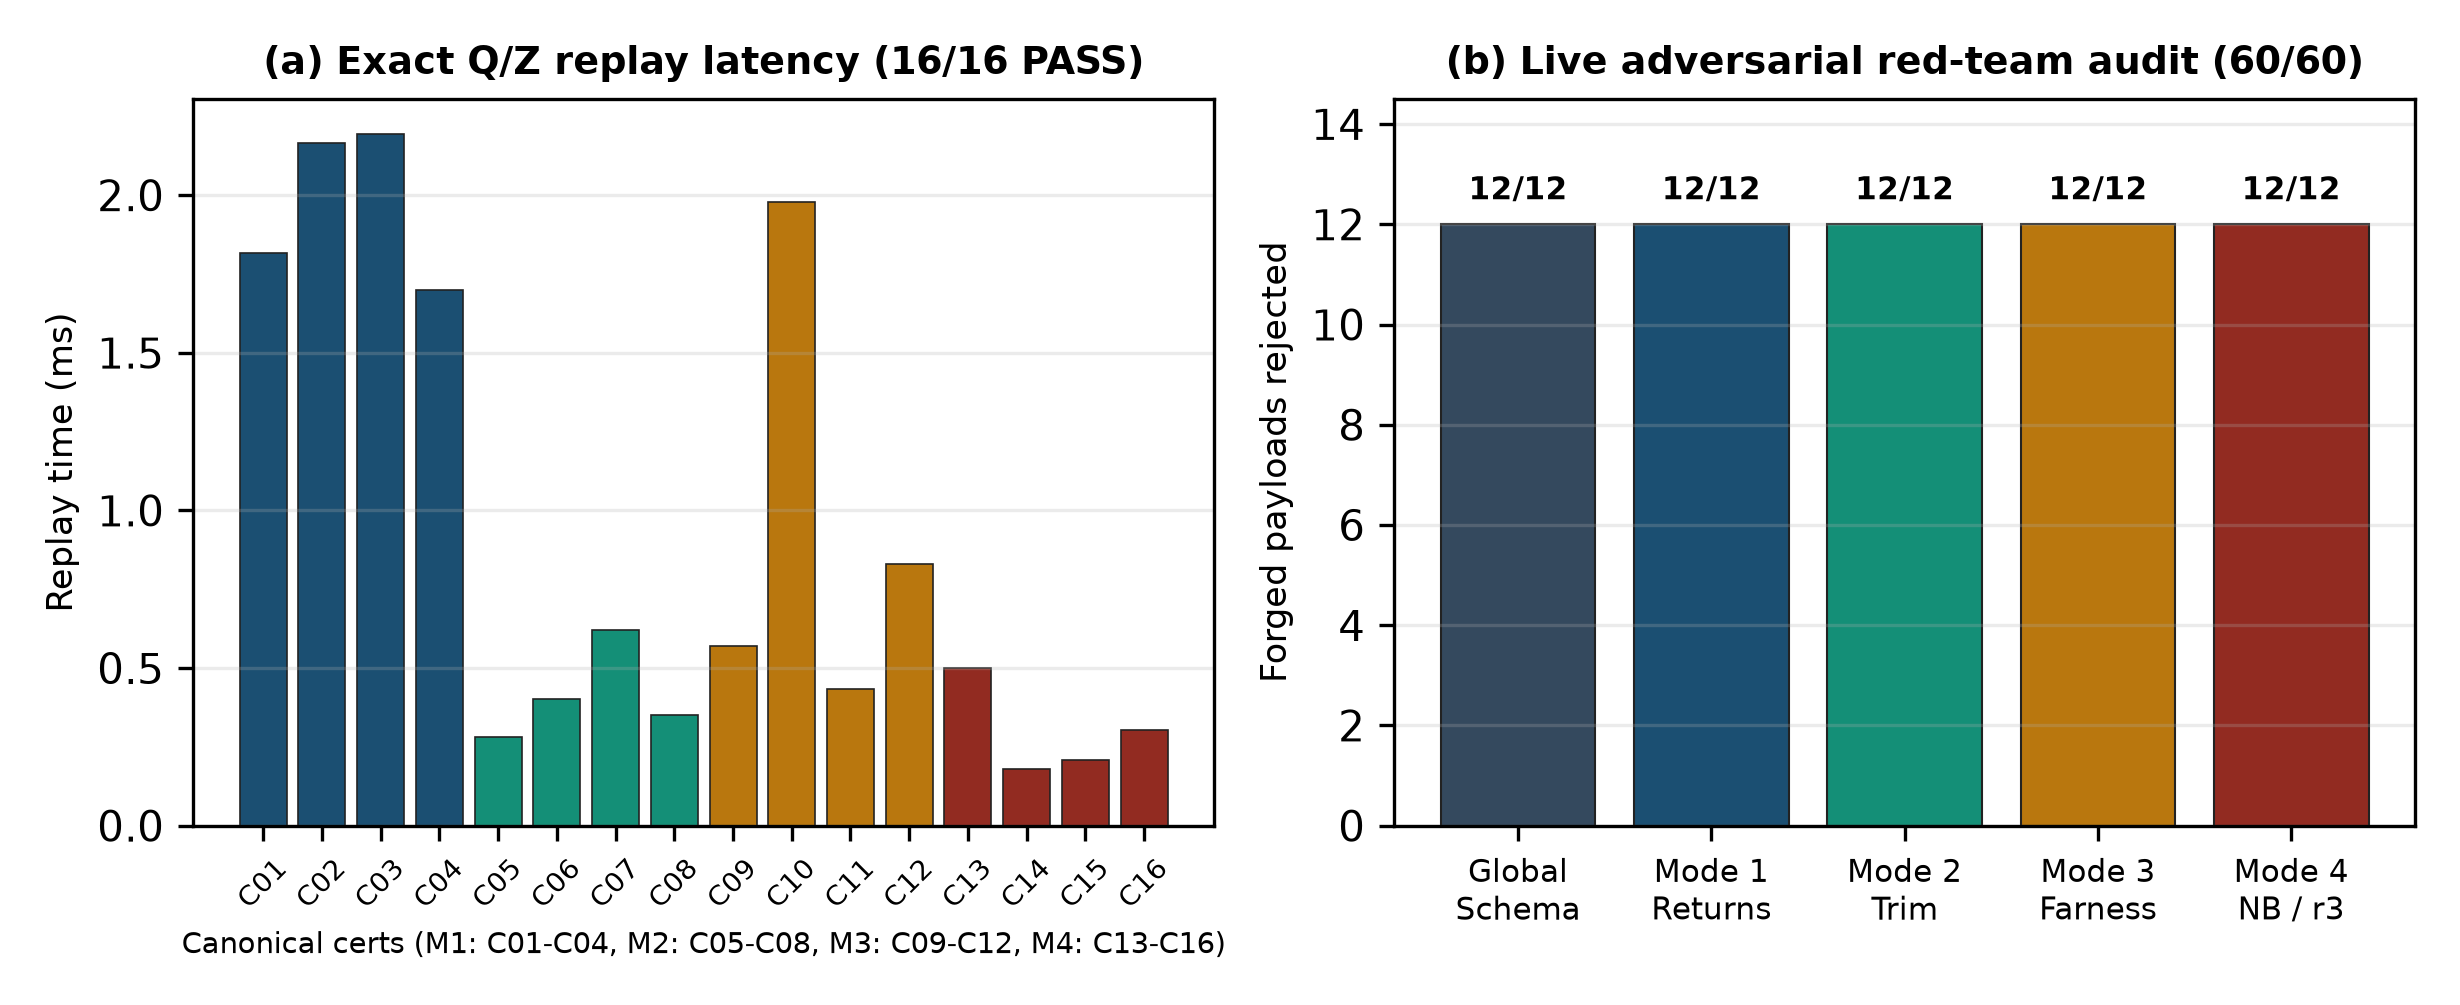
\includegraphics[width=\columnwidth]{../figures/fig3_certificate_replay_atlas.png}
  \caption{(a) Exact $\mathbb{Q}/\mathbb{Z}$ replay latency ($0.180$--$2.195\,\mathrm{ms}$) across all 16 canonical \texttt{EXP-RETPROB-CERT-1.0} certificates. (b) Live adversarial red-team audit rejecting 60/60 forged payloads across all five categories.}
  \label{fig:atlas}
\end{figure}

\paragraph{Replay Latency and 60/60 Red-Team Audit (Fig.~\ref{fig:atlas}).}
All 16 canonical certificates replay deterministically in $0.180$--$2.195\,\mathrm{ms}$ (total $14.53\,\mathrm{ms}$). The live adversarial suite (\texttt{tests/test\_suite.py}) tests 60 targeted forgeries---12 global schema/typing/canonical-rational/depth/control-char attacks plus 12 domain attacks per mode (self-loops, degree overflows, corrupted $A_s/B_s$, unsorted sets, invalid $h$-bounds, disconnected cuts, $c^* \le h_1$, non-regular $Q_k$, mismatched $r_3(4N)$, and identical $F_3$ pairs)---achieving \textbf{60/60 (100\%)} rejection.

\section{Conclusion}\label{sec:conc}
We delivered a standalone, zero-floating-point verification framework for Melissaris's return-probability expansion testing theory~\cite{melissaris2026testing}, combining 18 zero-\texttt{sorry}, zero-\texttt{Classical.choice} Lean~4.35.0 theorems with the exact $\mathbb{Q}/\mathbb{Z}$ verifier \texttt{EXP-RETPROB-CERT-1.0}, 16 canonical certificates, and 60/60 live adversarial forgery rejections.

\bibliographystyle{plain}
\bibliography{references}
\end{document}
